%% LyX 2.0.3 created this file.  For more info, see http://www.lyx.org/.
%% Do not edit unless you really know what you are doing.
\documentclass[english,11pt]{article}
\usepackage[T1]{fontenc}
\usepackage[latin9]{inputenc}
\setlength{\parskip}{\medskipamount}
\setlength{\parindent}{0pt}
\usepackage{babel}
\usepackage{float}
\usepackage{rotfloat}
\usepackage{amsthm}
\usepackage{amsmath}
\usepackage{graphicx}
\usepackage[unicode=true,pdfusetitle,
 bookmarks=true,bookmarksnumbered=false,bookmarksopen=false,
 breaklinks=false,pdfborder={0 0 0},backref=false,colorlinks=false]
 {hyperref}
\usepackage{breakurl}

\makeatletter
%%%%%%%%%%%%%%%%%%%%%%%%%%%%%% Textclass specific LaTeX commands.
\numberwithin{equation}{section}
\numberwithin{figure}{section}
\theoremstyle{plain}
\newtheorem{thm}{\protect\theoremname}
  \theoremstyle{definition}
  \newtheorem{defn}[thm]{\protect\definitionname}
  \theoremstyle{plain}
  \newtheorem{prop}[thm]{\protect\propositionname}
  \theoremstyle{plain}
  \newtheorem{conjecture}[thm]{\protect\conjecturename}

\@ifundefined{date}{}{\date{}}
%%%%%%%%%%%%%%%%%%%%%%%%%%%%%% User specified LaTeX commands.
\usepackage{tikz}
\usepackage{pgfplots}
\usetikzlibrary{arrows,automata,shapes,chains,positioning}

\usepackage{amsfonts}

% redefine ensuremath to put a space behind it
% this fixes broken LyX behavior that removes spaces behind it sometimes
\usepackage{xspace} % conditional spaceing
\let\Oldensuremath\ensuremath
\renewcommand{\ensuremath}[1]{\Oldensuremath{#1}\xspace}

\makeatother

  \providecommand{\conjecturename}{Conjecture}
  \providecommand{\definitionname}{Definition}
  \providecommand{\propositionname}{Proposition}
\providecommand{\theoremname}{Theorem}

\begin{document}


\global\long\def\Sym{\operatorname{Sym}}


\global\long\def\Aut{\operatorname{Aut}}


\global\long\def\Ker{\operatorname{Ker}}


\global\long\def\Img{\operatorname{Im}}


\global\long\def\Sep{\operatorname{Sep}}


\global\long\def\powerset{\operatorname{\mathcal{P}}}




\global\long\def\functionclass#1{\mathcal{#1}}


\global\long\def\FP{\functionclass{FP}}




\global\long\def\complexityclass#1{\mathrm{#1}}


\global\long\def\DTIME{\complexityclass{DTIME}}
\global\long\def\NTIME{\complexityclass{NTIME}}
\global\long\def\coNTIME{\complexityclass{coNTIME}}


\global\long\def\P{\complexityclass P}
\global\long\def\NP{\complexityclass{NP}}
\global\long\def\coNP{\complexityclass{coNP}}


\global\long\def\UP{\complexityclass{UP}}


\global\long\def\E{\complexityclass E}
\global\long\def\NE{\complexityclass{NE}}
\global\long\def\coNE{\complexityclass{coNE}}


\global\long\def\EE{\complexityclass{EE}}
\global\long\def\NEE{\complexityclass{NEE}}
\global\long\def\coNEE{\complexityclass{coNEE}}


\global\long\def\EEE{\complexityclass{EEE}}
\global\long\def\NEEE{\complexityclass{NEEE}}
\global\long\def\coNEEE{\complexityclass{coNEEE}}


\global\long\def\EXP{\complexityclass{EXP}}
\global\long\def\NEXP{\complexityclass{NEXP}}
\global\long\def\coNEXP{\complexityclass{coNEXP}}


\global\long\def\DisjNP{\complexityclass{DisjNP}}


\global\long\def\SPARSE{\complexityclass{SPARSE}}


\global\long\def\degree{\operatorname{d}}


\global\long\def\GI{\complexityclass{GI}}
\global\long\def\GNI{\complexityclass{GNI}}


\global\long\def\AM{\complexityclass{AM}}
\global\long\def\coAM{\complexityclass{coAM}}




\global\long\def\redmo{\leq_{m}^{p}}
\global\long\def\equivmo{\equiv_{m}^{p}}
\global\long\def\redmoneq{<_{m}^{p}}


\global\long\def\redt{\leq_{T}^{p}}
\global\long\def\equivt{\equiv_{T}^{p}}
\global\long\def\redtneq{<_{T}^{p}}




\global\long\def\predmo{\leq_{m}^{pp}}
\global\long\def\pequivmo{\equiv_{m}^{pp}}
\global\long\def\predmoneq{<_{m}^{pp}}


\global\long\def\predsmo{\leq_{sm}^{pp}}
\global\long\def\pequivsmo{\equiv_{sm}^{pp}}
\global\long\def\predsmoneq{<_{sm}^{pp}}


\global\long\def\predt{\leq_{T}^{pp}}
\global\long\def\pequivt{\equiv_{T}^{pp}}
\global\long\def\predtneq{<_{T}^{pp}}


\global\long\def\predunimo{\leq_{um}^{pp}}
\global\long\def\pequivunimo{\equiv_{um}^{pp}}
\global\long\def\predunimoneq{<_{um}^{pp}}


\global\long\def\predunit{\leq_{uT}^{pp}}
\global\long\def\pequivunit{\equiv_{uT}^{pp}}
\global\long\def\predunitneq{<_{uT}^{pp}}




\global\long\def\simp{\leq_{p}}




\global\long\def\lang#1{\mathrm{#1}}


\global\long\def\SAT{\lang{SAT}}
\global\long\def\SATstar{\lang{SAT}^{*}}


\global\long\def\REF{\lang{REF}}


\global\long\def\TAUT{\lang{TAUT}}


\global\long\def\TALLY{\lang{TALLY}}




\global\long\def\true{\text{true}}
\global\long\def\false{\text{false}}




\newcommand{\keyreturn}{return}


\title{Survey of Disjoint $\NP$-Pairs and Propositional Proof Systems }


\author{Nils Wisiol%
\thanks{University at Buffalo, New York, \texttt{mail@nils-wisiol.de}%
}}

\maketitle

\section{Introduction}



History of NP-Pairs and Propositional Proof Systems

CR79 program, ESY, ... ?

Razborov, ESY-Conjecture, Optimal Proof System for $\TAUT$?

\begin{sidewaysfigure}
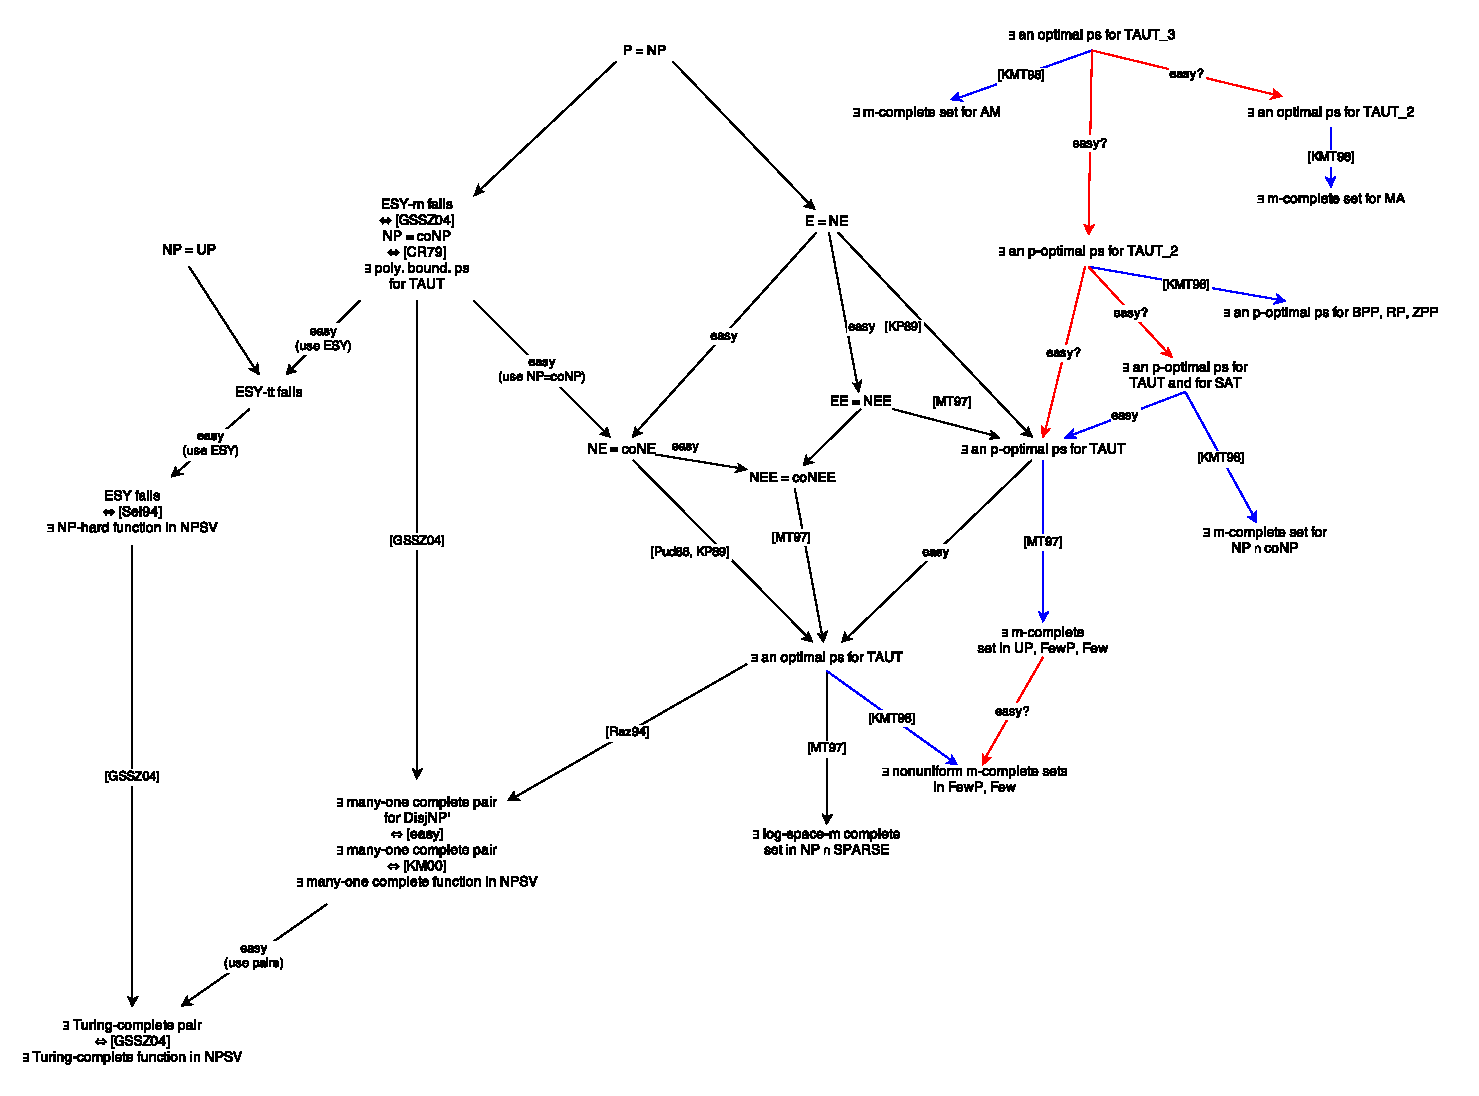
\includegraphics[width=1\textwidth]{implicationchart}

\caption{Known Implications for proof systems, disjoint pairs and the ESY conjecture
}
\end{sidewaysfigure}



\section{Preliminaries}


\subsection{Disjoint $\NP$-Pairs}

Disjoint NP-Pairs, Reductions

ESY-conjectures, ESY-m implies ESY-tt implies ESY-T

For two sets $A,B\in\NP$ that are disjoint, we call $(A,B)$ a \emph{disjoint
$\NP$-pair}. Following Grollmann and Selman \cite{journals/siamcomp/GrollmannS88},
we use the following reductions of $\NP$-pairs, that naturally arise
from the reductions of languages.
\begin{defn}

\begin{enumerate}
\item $(A,B)$ is \emph{many-one-reducible in polynomial time} to $(C,D)$,
$(A,B)\predmo(C,D)$, if for every separator $T\in\Sep(C,D)$, there
exists a separator $S\in\Sep(A,B)$ such that $S\redmo T$.
\item $(A,B)$ is \emph{many-one-reducible in polynomial time} to $(C,D)$,
$(A,B)\predt(C,D)$, if for every separator $T\in\Sep(C,D)$, there
exists a separator $S\in\Sep(A,B)$ such that $S\redt T$.
\end{enumerate}
\end{defn}
1-invertible, many-one, smart Turing, Turing, truth-table, bounded-truth-table
reductions, strongly many-one reduction

Analog to languages, we define completeness for disjoint $\NP$-pairs.
\begin{defn}

\begin{enumerate}
\item A pair $(A,B)$ is $\predmo$-complete, if for every $(C,D)\in\DisjNP$
we have $(C,D)\predmo(A,B)$.
\item A pair $(A,B)$ is $\predt$-complete, if for every $(C,D)\in\DisjNP$
we have $(C,D)\redt(A,B)$.
\end{enumerate}
\end{defn}
\begin{prop}

\begin{enumerate}
\item $(A,B)\redt(C,D)$ if and only if $(A,B)\predunit(C,D)$. \cite{journals/siamcomp/GrollmannS88}
\item $(A,B)\redmo(C,D)$ if and only if $(A,B)\predunimo(C,D)$. \cite{journals/eccc/ECCC-TR03-011}
\end{enumerate}
\end{prop}

\subsubsection{ESY-conjectures}

We state the original ESY-conjecture \cite{journals/iandc/EvenSY84}
as well as the many-one version \cite{conf/icalp/HughesPRS12} of
it. The many-one version of the conjecture was proven to be equivalent
to $\NP\neq\coNP$ by Gla�er et al. \cite{journals/eccc/ECCC-TR03-011}.
\begin{conjecture}[ESY]
 For every pair of disjoint sets in $\NP$, there is a separator
that is not Turing-hard for $\NP$.
\end{conjecture}

\begin{conjecture}[ESY-m]
 For every pair of disjoint sets in $\NP$, there is a separator
that is not many-one-hard for $\NP$.
\end{conjecture}

\subsection{Propositional Proof Systems}

A propositional proof system is a fast method of verifying proofs.

To give an example, we will have a look at the \emph{resolution principle},
which was introduced by Robinson \cite{journals/jacm/Robinson65}.
Consider a boolean formula $\varphi$ in conjunctive normal form.
If $\varphi$ is not satisfiable, the resolution principle provides
a way to find a proof for this fact. To find a proof, the resolution
principle iteratively combines two existing clauses into a new and
shorter clause with equivalent truth value. Robinson showed that the
resolution principle yields the empty clause eventually for any unsatisfiable
formula, and any formula for which the principle yields the empty
clause is unsatisfiable:
\begin{thm}[Resolution Theorem \cite{journals/jacm/Robinson65}]
\label{thm:resolution-theorem} For a formula $\varphi$ in conjunctive
normal form, the resolution principle yields the empty clause if and
only if $\varphi$ is not satisfiable.
\end{thm}
As we can see from the way resolution works, there are exponentially
many options how to combine the clauses, and not every sequence of
combinations will yield the empty clause. Hence, it is hard to find
a sequence of combinations that derive the empty clause. By Theorem
\ref{thm:resolution-theorem}, this sequence exists if and only if
the formula is unsatisfiable. As opposed to finding a sequence, given
a sequence of combinations, we can easily check if this sequence derives
the empty clause.

Using formal terms, let $f$ be defined by
\[
f(\langle\varphi,w\rangle)=\begin{cases}
\neg\varphi & \text{if combination sequence \ensuremath{w}applied to \ensuremath{\varphi}yields the empty clause,}\\
\perp & \text{otherwise.}
\end{cases}
\]
Intuitively, $f$ is polynomial-time computable. By the Resolution
Theorem, $f$ only outputs tautologies, and for every tautology $\neg\varphi$,
there is an input $\langle\varphi,w\rangle$ such that $f(\langle\varphi,w\rangle)=\neg\varphi$. 

Given a combination sequence $w$ that yields the empty clause for
$\varphi$, the function $f$ provides a fast way to verify $\neg\varphi$
is a tautology. We thus call $f$ a propositional proof system, and
we call $\langle\varphi,w\rangle$ a $f$-proof for $\neg\varphi$.
\begin{defn}
A polynomial-time computable function $f$ that is onto the set of
tautologies is called a \emph{propositional proof system} or \emph{proof
system}. For any $w$, we say $w$ is a \emph{$f$-proof for $x$}
if $f(w)=x$. If there is a polynomial $p$, such that for all $x$,
and all $f$-proofs $w$ of $x$, we have $|w|\leq p(|x|)$, then
$f$ is \emph{polynomially-bounded}.
\end{defn}


Cook and Reckhow started a line of research \cite{journals/jsyml/CookR79}
that tries to investigate what the length of the shortest proof of
a propositional tautology relative to the length of the tautology
is. The interest in the length of the proof is motivated by the fact
that the existence of polynomial-length proofs for all tautologies
characterizes the question of whether $\NP=\coNP$. (A fact we will
prove in section \ref{sec:Propositional-Proof-Systems}.) However,
no known proof system could be proven to have proofs with length bounded
by a polynomial. To tackle the problem, Cook and Reckhow introduced
the notion of simulation of proof systems.
\begin{defn}
Let $f$ and $g$ be proof systems. We say $f$ \emph{simulates} $g$,
if there is a function $h$ such that for all $w$, it holds $f(h(w))=g(w)$
and $|h(w)|\leq p(|w|)$. If $h$ is polynomial-time computable, we
say $f$ \emph{p-simulates} $g$. A proof system that simulates (p-simulates)
every other proof system is called \emph{optimal} (\emph{p-optimal}).
\end{defn}
An more intuitive (and informal) way to give a definition for ``$f$
simulates $g$'' is to say that for every tautology $\varphi$, the
$f$-proof for $\varphi$ is at most polynomially longer than the
$g$-proof of $\varphi$. An optimal proof system then has the shortest
proofs for tautologies among all proof systems, within a polynomial
factor.

However, it is not only unknown whether polynomially-bounded proof
systems exist, it is also unknown if optimal or even p-optimal proof
systems exist. To study the existence of optimal and p-optimal proof
systems, we will therefore study sufficient conditions and implications
in section \ref{sec:Propositional-Proof-Systems}. To become familiar
with the notions, we present a strong sufficient condition for the
existence of optimal proof systems:
\begin{thm}
\label{thm:np-eq-conp-implies-optimalpps}If $\NP=\coNP$, then there
is an optimal proof system.\end{thm}
\begin{proof}
Let $N$ be a $\NP$-machine deciding $\TAUT\in\coNP$. We define
$f$ by 
\[
f(\langle i,x\rangle)=\begin{cases}
x & \text{if \ensuremath{N}accepts \ensuremath{w}along path \ensuremath{i},}\\
\perp & \text{otherwise}.
\end{cases}
\]
Notice, a proof system does not have to be a total function. By definition,
$f$ outputs only tautologies, and for every tautology there is an
accepting path of $N$, so $f$ is onto $\TAUT$.

To see $f$ is optimal, let $f'$ be an arbitrary proof system. There
is a function $g$ mapping each tautology $w$ to an accepting path
$i$ of $N$. Notice, $g$ might not by polynomial-time computable,
but is polynomially length bounded. Let now $w$ be a $f'$-proof
for $x$. With $g$, we can translate $w$ into $\langle g(w),f'(w)\rangle$,
which is a $f$-proof for $x$.
\end{proof}
As we will see in section \ref{sec:Propositional-Proof-Systems},
the existence of both optimal and p-optimal proof systems can be proven
under much weaker hypotheses.


\section{Disjoint $\NP$-Pairs}


\subsection{Characterization of $\NP=\coNP$}
\begin{thm}
\cite{journals/eccc/ECCC-TR03-011}\label{thm:equiv-esymfails-np=00003Dconp-polyboundpps}The
following assertions are equivalent.
\begin{enumerate}
\item The ESY-m conjecture does not hold, that is, there exists a disjoint
$\NP$-pair such that all separators are many-one-hard for $\NP$.
\item $\NP=\coNP$
\end{enumerate}
\end{thm}

\subsection{Existence of Complete Pairs}

if ESY does not hold, this implies the existence of complete pairs.

\pagebreak{}


\section{Propositional Proof Systems\label{sec:Propositional-Proof-Systems}}


\subsection{Polynomially-bounded proof systems and $\NP=\coNP$}

Here will show that the existence of polynomially-bounded proof systems
characterizes $\NP=\coNP$. The proof is due to Cook and Reckhow \cite{journals/jsyml/CookR79}.
\begin{thm}
\label{thm:poly-bounded-ps-iff-np-eq-conp}There is a polynomially-bounded
propositional proof system if and only if $\NP=\coNP$.\end{thm}
\begin{proof}
Assume $\NP=\coNP$. Then there is an $\NP$-machine $M$ such that
for every tautology $\varphi$ there is an accepting path $w$ in
the computation of $M$. This allows us to define a proof system $f$,
in which all proofs are polynomially length bounded:
\[
f(\langle\varphi,w\rangle)=\begin{cases}
\varphi & \text{if \ensuremath{M}accepts \ensuremath{\varphi}on path \ensuremath{w}},\\
\true & \text{otherwise}.
\end{cases}
\]
Since $f$ only considers one path in the computation of $M$, it
is polynomial-time computable. Also, $f$ only outputs tautologies.
Therefore, $f$ is a proof system. As there is an accepting path in
the computation of $M$ for every tautology $\varphi$, all tautologies
have polynomial-length proofs.

To prove the converse, suppose there is a polynomially-bounded proof
system $f$. Since the complement of $\TAUT$ is $\NP$-complete,
it suffices to show $\TAUT\in\NP$. Let $M$ be a nondeterministic
Turing machine such that on input $\varphi$, $M$ guesses a $f$-proof
$w$ and calculates $f(\langle\varphi,w\rangle)$. The machine then
accepts if and only if $f(\langle\varphi,w\rangle)=\varphi$. Hence,
every accepted string is a tautology, and every tautology is accepted.
\end{proof}
To prove $\NP\neq\coNP$, that is, to prove there is no polynomially-bounded
proof system, Cook and Reckhow introduced the notion of optimal proof
systems. We call a proof system $f$ optimal, if $f$-proofs are the
shortest proofs among all proof systems (with respect to a polynomial
factor). If we could prove the existence of an optimal proof system
with proofs that are not within polynomial length, we could prove
$\NP\neq\coNP$.

However, it is unknown whether or not optimal proof systems with proofs
of any length exist, however a few necessary and sufficient conditions
are known.  


\subsection{Sufficient Conditions for the Existence}

To investigate further the question of whether optimal or even p-optimal
proof systems exist, first Kraj�\v{c}ek and Pudl�k \cite{journals/jsyml/KrajicekP89}
and later Me�ner and Tor�n prove sufficient conditions for the existence
of such proof systems. The results reveal a symmetry for sufficient
conditions for optimal and p-optimal proof systems:

\begin{figure}[H]
\begin{center}
\begin{tikzpicture}[->,>=stealth',shorten >=1pt,node distance=4.5cm,       semithick, /tikz/initial text=]   
\tikzstyle{every state}=[fill=none,draw=black,text=black]
  
\node (A0)               {$\P=\NP$};   
\node (B0) [right of=A0] {$\E=\NE$};
\node (C0) [right of=B0] {$\EE=\NEE$};
\node (D0) [right of=C0,align=center] {$\exists$ an p-optimal\\proof system};

\node (A1) [below=1cm of A0] {$\NP=\coNP$};   
\node (B1) [right of=A1] {$\NE=\coNE$};
\node (C1) [right of=B1] {$\NEE=\coNEE$};
\node (D1) [right of=C1,align=center] {$\exists$ an optimal\\proof system};

\path[every node/.style={sloped,anchor=south,auto=false}]
 (A0) edge (B0)
 (B0) edge (C0)
 (C0) edge (D0)

 (A1) edge (B1)
 (B1) edge (C1)
 (C1) edge (D1)

 (A0) edge (A1)
 (B0) edge (B1)
 (C0) edge (C1)
 (D0) edge (D1)
;
\end{tikzpicture}
\end{center}

\caption{The symmetric structure of sufficient conditions for optimal and p-optimal
propositional proof systems.}
\end{figure}


We call a language $L$ \emph{almost-tally}, if every string in $L$
is of the form $0^{*}10^{*}$. By $\powerset(0^{*}10^{*})$ we denote
the class of all almost-tally languages. Me�ner and Tor�n use the
notion of almost-tally languages to obtain an even weaker sufficient
condition than mentioned in the chart:
\begin{thm}
\label{thm:sufficient-cond-for-optimal-pps}
\begin{enumerate}
\item If all almost-tally languages in $\coNEE$ also belong to $\EE$,
then there exists a p-optimal propositional proof system.
\item If all almost-tally languages in $\coNEE$ also belong to $\NEE$,
then there exists an optimal propositional proof system.
\end{enumerate}
\end{thm}
The proof is based on constructing the almost-tally language $T$
which is, by definition, in $\coNEE$. By the hypothesis, we can then
assume $T\in\EE$ and $T\in\NEE$ respectively and define a proof
system based on $T$.

For the proof of \ref{thm:sufficient-cond-for-optimal-pps}.1, please
refer to the original paper by Me�ner and Tor�n \cite{journals/eccc/ECCC-TR97-026}.
\begin{proof}[Proof of \ref{thm:sufficient-cond-for-optimal-pps}.2]
Let $M_{1},M_{2},...$ be an enumeration of deterministic Turing
machines such that there is a universal Turing machine that can simulate
$k$ steps of $M_{i}$ in $(ik)^{2}$ steps. Define the almost-tally
language 
\begin{eqnarray*}
T=\{0^{j}10^{i} & \mid & \text{for all words \ensuremath{w}of length at most \ensuremath{2^{2^{j+1+i}}}:}\\
 &  & (\text{if \ensuremath{M_{i}}halts on \ensuremath{w}in at most \ensuremath{2^{2^{j+1+i}}}steps, then \ensuremath{M_{i}}outputs a tautology})\}.
\end{eqnarray*}
To see that $T$ is a $\coNEE$-language, we rewrite $T$ as 
\begin{eqnarray*}
T=\{0^{j}10^{i} & \mid & \forall w,y\in\Sigma^{\leq2^{2^{j+1+i}}}:\\
 &  & \left[M_{i}(w)\text{ halts in \ensuremath{2^{2^{j+1+i}}}steps }\implies(M_{i}(w)=\varphi\wedge\varphi(y)=\true)\right]\},
\end{eqnarray*}
where the condition written in square brackets can be decided in deterministic
double-exponential time. By the hypothesis, we thus have $T\in\NEE$.
Let $N_{T}$ denote the nondeterministic Turing machine deciding $T$
in time $2^{c2^{n}}$, $c\geq1$.

Based on $N_{T}$, we will now define a proof system $f$, 
\[
f(\langle0^{j}10^{i},0^{s},\alpha,w\rangle)=\begin{cases}
M_{i}(w) & \text{if for \ensuremath{l=j+1+i}all of the following requirements are met:}\\
 & \text{(a) \ensuremath{s\geq2^{2^{l}}}},\\
 & \text{(b) \ensuremath{|w|\leq2^{2^{l}}}},\\
 & \text{\text{(c) \ensuremath{M_{i}}on input \ensuremath{w}halts in at most \ensuremath{2^{2^{l}}}steps},}\\
 & \text{(d) \ensuremath{\alpha}is an accepting computation of \ensuremath{N_{T}}on input \ensuremath{0^{j}10^{i}}},\\
\true & \text{otherwise.}
\end{cases}
\]
First, we will show that $f$ is a proof system. In both cases of
the definition, $f$ only outputs tautologies. Also, for any given
tautology $\varphi$, there is a $k$ such that $M_{k}$ outputs $\varphi$
on any input with length at least $|\varphi|$, and true for all shorter
inputs. Hence $10^{k}\in T$. Therefore, there is an $\alpha$ such
that $\langle10^{k},0^{2^{2^{k+1}}},\alpha,0^{|\varphi|}\rangle$
is a $f$-proof for $\varphi$. This confirms $f(\Sigma^{*})=\TAUT$.
As a last condition, we need to verify $f$ is polynomial-time computable:
a machine computing $f$ first checks if $s\geq2^{2^{l}}$. If this
is true, conditions (b), (c) and (d) can be verified in polynomial-time
in $|0^{s}|$. If the check exceeds the polynomial-time limit, condition
(a) does not hold and $\true$ will be output. Hence, $f$ is polynomial-time
computable.

To demonstrate that $f$ is an optimal proof system, let $g$ be any
other proof system. For a given $g$-proof $w$, where $g$ is computed
by transducer $M_{i}$ with time bound $n^{k}+k$, we will see that
there is an $\alpha$ such that 
\begin{eqnarray*}
w' & = & \langle0^{j}10^{i},0^{s},\alpha,w\rangle,\text{ where}\\
s & = & 2^{c2^{j+1+i}}\\
j & = & \max(0,\left\lceil \log\log\left(|w|^{k}+k\right)\right\rceil -i-1)
\end{eqnarray*}
is an $f$-proof for the same tautology, because the string $w'$
satisfies all conditions in the first case of the definition of $f$,
and therefore $f(w')=M_{i}(w)=g(w)$: (a) is satisfied by the choice
of $s$, (b) holds by the choice of $j$: We distinguish two cases.
\begin{eqnarray*}
\text{If }j>0, &  & 2^{2^{l}}=2^{2^{\left\lceil \log\log\left(|w|^{k}+k\right)\right\rceil }}\geq2^{2^{\log\log\left(|w|^{k}+k\right)}}=|w|^{k}+k\geq|w|.\\
\text{If }j=0, &  & \left\lceil \log\log\left(|w|^{k}+k\right)\right\rceil -i-1\leq0\implies\left\lceil \log\log\left(|w|^{k}+k\right)\right\rceil \leq i+1\\
 &  & \implies\log\log\left(|w|^{k}+k\right)\leq i+1\implies|w|^{k}+k\leq2^{2^{i+1}}=2^{2^{l}}\implies|w|\leq|w|^{k}+k\leq2^{2^{l}}.
\end{eqnarray*}
Condition (c), again, holds by choice of $j$: The runtime of $M_{i}$
on input $w$ is bounded by $|w|^{k}+k$, which is, as we have just
seen, in both cases less or equal than $2^{2^{l}}$. For condition
(d), remember that $M_{i}$ is computing a proof system and thus only
outputs tautologies, which implies $0^{j}10^{i}\in T$. Therefore,
there is an $\alpha$ that is an accepting computation of $N_{T}$
on input $0^{j}10^{i}$.

It remains to show that $|w'|\leq p(|w|)$. To see this, it is sufficient
to show that $j$, $i$, $s$ and $\alpha$ are polynomial in $|w|$.
$j$ is indeed double-logarithmic, and thus $s$ is polynomial in
$|w|$. The G�del-number $i$ is a constant in $|w|$. The computation
path $\alpha$ has double-exponential length in $i$ and $j$ and
therefore polynomial in $|w|$.
\end{proof}

\subsection{Implications of the Existence}

In this section, we will see some evidence suggesting optimal proof
systems do not exist. One of the implications given by optimal proof
systems is the existence of complete sets for $\NP\cap\SPARSE$, a
consequence which we tend to believe is not true. This result is due
to K�bler et al \cite{journals/iandc/KoblerMT03}. However our interest
in this result goes beyond this evidence, as Buhrman et al. \cite{conf/stacs/BuhrmanFFM00}
showed that there is an oracle such that there are no complete sets
for $\NP\cap\SPARSE$, although oracles to which there are no optimal
proof systems have been known even before that \cite{journals/jsyml/KrajicekP89,journals/iandc/KoblerMT03}.
\begin{thm}
If there is an optimal proof system, then complete sets for $\NP\cap\SPARSE$
exist.\end{thm}
\begin{proof}
We define the set $SP$, containing descriptions of non-deterministic
Turing machines that have runtime bounded by $l$ and accept, up to
a given length $n$, only $l$ different strings: 
\begin{eqnarray*}
 & SP=\{\langle N,0^{l},0^{n}\rangle\mid & \text{(1)}\, N\,\text{is a non-deterministic Turing machine}\\
 &  & \text{\text{(2) there are at most \ensuremath{l}pairs \ensuremath{(x_{i},y_{i})}such that}}\\
 &  & \qquad\text{(a) all \ensuremath{x_{i}}are different}\\
 &  & \qquad\text{(b) all \ensuremath{y_{i}}are different }\\
 &  & \qquad\text{(c) }|x_{i}|\leq n,|y_{i}|\leq l\\
 &  & \qquad\text{(d) \ensuremath{N}accepts \ensuremath{x_{i}}on path \ensuremath{y_{i}}}\}
\end{eqnarray*}
 $\overline{SP}$ therefore holds all tuples $\langle N,0^{l},0^{n}\rangle$
such that there exists $l+1$ inputs $x_{i}$ of length at most $n$
that are accepted by $N$, which proves that $SP\in\coNP$.

We will now define subsets of $SP$ that can be decided in deterministic
polynomial time. Assume $M$ is a non-deterministic Turing machine
with polynomial runtime $q$ such that for every $n$, $M$ accepts
at most $q(n)$ strings of length at most $n$. That is, the language
accepted by $M$, $L(M)$ is $q$-sparse. Note that the set $SP_{M}=\{\langle M,0^{q(n)},0^{n}\rangle\mid n\geq1\}$
is a subset of $SP$. For every such $M$, there is a deterministic
polynomial-time Turing machine $T_{M}$ that decides $SP_{M}$: given
an input $\langle N,0^{l},0^{n}\rangle$, it checks whether $N=M$
and $l=q(n)$, where $M$ and $q$ are coded into $T_{M}$'s program.
We will use $SP_{M}$ later to show the completeness.

We are going to define the set $S\in\NP\cap\SPARSE$, and prove it
is complete for that class. The fact that there is an optimal proof
system will yield the many-one reduction. So let $h$ be an optimal
proof system and let $SP$ reduce to $TAUT$ via $\gamma,$ which
gives us $z\in SP\iff\gamma(z)\in TAUT$. Then we define 
\begin{eqnarray*}
 & S=\{\langle0^{N},0^{j},x\rangle\mid & \text{(I) \ensuremath{N}is non-det. Turing machine}\\
 &  & \text{(II) there exists \ensuremath{w}, \ensuremath{|w|\leq j}},\\
 &  & \qquad\text{(a) }h(w)=\gamma(\langle N,0^{l},0^{|x|}\rangle),\\
 &  & \qquad\text{(b) \ensuremath{N}accepts \ensuremath{x}in at most \ensuremath{l}steps}.\}
\end{eqnarray*}
We can see $S$ belongs to $\NP$ because of the polynomial-time condition
on the tuple. To see $S$ is sparse, first fix an $N$ and $j$. By
condition (II)(b), every $x$ such that $\langle0^{N},0^{j},x\rangle\in S$
is accepted by $N$ in at most $l$ steps. Since $\langle N,0^{l},0^{|x|}\rangle\in SP$
by (II)(a), we have $N$ only accepting at most $l$ inputs of length
at most $|x|$. For the fixed $N$ and $j$ we thus have at most $l$
tuples $\langle0^{N},0^{j},x\rangle\in S$. By condition (II)(a),
we can relate this upper bound to the length of the tuples: since
$h$ and $\gamma$ are both polynomial length bounded, $l$ is bounded
by some polynomial in $j$. Therefore exist for any given $N$ and
$j$ only a in $j$ polynomial number of tuples in $S$. By the tally
encoding of $N$ and $j$, there exist only a polynomial number of
different $N$ and $j$ for any fixed length $k$ of tuples in $S$.

Now let's see how every set in $\NP\cap\SPARSE$ many-one reduces
to $S$. Let $S'$ be a set in $\NP\cap\SPARSE$ that is accepted
by $M$ in time $q$. As shown before, $SP_{M}$ can then be decided
in polynomial time. This enables us to define a polynomial-time function
\[
g_{M}(x)=\begin{cases}
\gamma(x) & \text{if \ensuremath{x\in SP_{M},}}\\
\perp & \text{otherwise}
\end{cases}
\]
with range $\TAUT$. That is, $g_{M}$ is a proof system and thus
simulated by the optimal proof system $h$. Hence, there exists a
translation function $\lambda$ and a polynomial $r$ such that for
all $g_{M}$-proofs $x$, we have $h(\lambda(x))=g_{M}(x)$ and $|\lambda(x)|\leq r(|x|)$.
We can thus reduce $S'$ to $S$ via the polynomial-time function
$x\mapsto\langle0^{M},0^{r(|x|)},x\rangle$. 

To prove this claim, assume $x\in S'$. By definition we have $z=\langle M,0^{q(|x|)},0^{|x|}\rangle\in SP_{M}$.
Thus, $z$ is a $g_{M}$-proof for $\gamma(z)$, and therefore $\lambda(z)$
is an $h$-proof for $\gamma(z)$, so $w=\lambda(z)$ satisfies condition
(II)(a). Condition (I) of $S$ is fulfilled by definition. For the
length bound of (II), notice $|w|=|\lambda(z)|\leq r(|x|)=j$. Since
$\lambda(z)$ is an $h$-proof for $\gamma(z)$, we have $z=\langle N,0^{l},0^{|x|}\rangle\in SP$.
We thus know by definition of $SP$ that $N$ accepts inputs of length
at most $|x|$ in at most $l$ steps. This satisfies condition (II)(b).
Altogether, we have $\langle0^{M},0^{r(|x|)},x\rangle\in S$. The
converse follows immediately from (II)(b).
\end{proof}
The technique of this proof can be generalized and extended to a lot
of promise classes, most interestingly $\UP$:
\begin{thm}

\begin{enumerate}
\item If there is an p-optimal proof system, then $\UP$ has a many-one
complete set.
\item If there is an optimal proof system, then $\UP$ has a complete set
under non-uniform many-one reducibility.
\end{enumerate}
\end{thm}
For the proof, we refer the reader to the work of K�bler, Me�ner and
Tor�n \cite{journals/iandc/KoblerMT03}. Among $\UP$, it also contains
results on 

One of the most outstanding consequence of the existence of optimal
proof systems is the existence of complete $\NP$-pairs, first proven
by Razborov in 1994. The proof requires some preparation and is demonstrated
in the next section.

\pagebreak{}


\section{Propositional Proof Systems and $\NP$-Pairs}




\subsection{Canonical Pairs}

Simulation of Proof Systems and Reduction of Canonical Pairs

Razborov


\section{Relativized Worlds}


\subsection{No Optimal/p-Optimal Proof System}

Optimal: paper by Fortnow et al; p-optimal: paper by Me�ner Tor�n 


\subsection{Converse of Razborov does not Hold}

paper by Gla�er et al. (GSSZ section 6)


\subsection{ESY holds}

paper by GSSZ section 3


\subsection{Separation of ESY refinements}

ask Andy (meeting with Lance: there is an oracle such that $\NP=\UP$
and $\NP\neq\coNP$.


\section{Conclusion}




\subsection{Open Questions and Future Work}
\begin{enumerate}
\item Oracle for which converse of Razborov holds
\item Oracle such that there is a optimal, but not a p-optimal proof system
\end{enumerate}
\bibliographystyle{alpha}
\bibliography{bibliography}

\end{document}
